
\documentclass[intern]{cgMA}

\usepackage{csquotes} % Für \enquote
% Dokumentation: https://www.namsu.de/Extra/pakete/Csquotes.html
\usepackage{subcaption} % subfigure/subcaption Umgebungen und \subcaption Befehl
\usepackage{hyperref} % Macht automatisch klickbare Links bei Referenzen etc.
\usepackage{listings} % Für Code-listings o.ä.
\usepackage{graphicx} % Für Graphiken
\usepackage{amsmath,amssymb,amsfonts} % Mathe, Symbole....
\DeclareMathOperator{\Tr}{Tr}
\usepackage{algpseudocode}
\usepackage{algorithm}
\usepackage{float}
\usepackage{gensymb} % Mathe, Symbole....
\usepackage{textcomp} % Symbole....
\usepackage{bm} % \bm{x} Befehl um in Mathe fett zu setzen
\usepackage{cleveref}
\usepackage{blindtext}
\usepackage{titlesec}
\usepackage[symbols,nogroupskip,record,toc=false]{glossaries-extra}
\nocite{*}
\usepackage[
    backend=biber,
    style=ieee,
    dashed=false,
    sortlocale=en_US,
    natbib=true,
    url=true, 
    doi=true,
    eprint=false
]{biblatex}
\addbibresource{sources.bib}

\title{Real-time Simulation of Granular Matter using Smoothed Particle Hydrodynamics}
\author{André Neder}
\zweitgutachter{Alexander Maximilian Nilles, M.Sc.}
\zweitgutachterInfo{(Institut für Computervisualistik, AG Computergraphik)}
% \externLogo{7.46cm}{logos/ExternLogoPlaceholder}
% \externName{DIN: NewTechnologies}

\glsxtrnewsymbol[description={particle index}]{i, j}{\ensuremath{i}, \ensuremath{j}}
\glsxtrnewsymbol[description={boundary index}]{b}{\ensuremath{b}}
\glsxtrnewsymbol[description={iteration index}]{l}{\ensuremath{l}}
\glsxtrnewsymbol[description={density}]{rho}{\ensuremath{\rho}}
\glsxtrnewsymbol[description={pressure}]{p}{\ensuremath{p}}
\glsxtrnewsymbol[description={friction}]{f}{\ensuremath{p}}
\glsxtrnewsymbol[description={position}]{x}{\ensuremath{x}}
\glsxtrnewsymbol[description={velocity}]{v, u}{\ensuremath{v}, \ensuremath{u}}
\glsxtrnewsymbol[description={force}]{F}{\ensuremath{F}}
\glsxtrnewsymbol[description={time}]{t}{\ensuremath{t}, \ensuremath{\Delta t}}
\glsxtrnewsymbol[description={mass}]{m}{\ensuremath{m}}
\glsxtrnewsymbol[description={volume}]{V}{\ensuremath{V}}
\glsxtrnewsymbol[description={strain}]{varepsilon}{\ensuremath{\varepsilon}}
\glsxtrnewsymbol[description={stress}]{s}{\ensuremath{s}}
\glsxtrnewsymbol[description={strain to stress relation tensor}]{D}{\ensuremath{D}}
\glsxtrnewsymbol[description={gradient operator}]{nabla}{\ensuremath{\nabla}}
\glsxtrnewsymbol[description={dynamic viscosity}]{mu}{\ensuremath{\mu}}
\glsxtrnewsymbol[description={an arbitrary field}]{H}{\ensuremath{H}}
\glsxtrnewsymbol[description={particle radius}]{r}{\ensuremath{r}}
\glsxtrnewsymbol[description={a kernel function}]{W, w}{\ensuremath{W}, \ensuremath{w}}
\glsxtrnewsymbol[description={cubic spline kernel function}]{C(x)}{\ensuremath{C(x)}}
\glsxtrnewsymbol[description={kernel radius (smoothing length)}]{h}{\ensuremath{h}}
\glsxtrnewsymbol[description={distance between two particles}]{delta}{\ensuremath{\delta}}
\glsxtrnewsymbol[description={surface normal}]{n}{\ensuremath{n}}
\glsxtrnewsymbol[description={frictional coefficient}]{alpha}{\ensuremath{\alpha}}
\glsxtrnewsymbol[description={angle of repose}]{theta}{\ensuremath{\theta}}
\glsxtrnewsymbol[description={stiffness parameters}]{k, B, gamma}{\ensuremath{k}, \ensuremath{B}, \ensuremath{\gamma}}
\glsxtrnewsymbol[description={cubic extension function}]{gamma*}{\ensuremath{\gamma^*}}
\glsxtrnewsymbol[description={relaxation factor}]{omega}{\ensuremath{\omega}}
\glsxtrnewsymbol[description={IISPH coefficient}]{a_ii}{\ensuremath{a_{ii}}}
\glsxtrnewsymbol[description={displacement of i due to pressure j}]{d_{ij}p_{j}}{\ensuremath{d_{ii}p_{i}}}
\glsxtrnewsymbol[description={signed distance function}]{Phi}{\ensuremath{\Phi}}
\glsxtrnewsymbol[description={blending weight}]{eta}{\ensuremath{\eta}}
\glsxtrnewsymbol[description={maximum compression}]{lambda}{\ensuremath{\lambda}}
\glsxtrnewsymbol[description={helper variable}]{psi}{\ensuremath{\psi}}
\glsxtrnewsymbol[description={occlusion weight}]{Omega}{\ensuremath{\Omega}}
\glsxtrnewsymbol[description={crosssectional area}]{A}{\ensuremath{A}}
\glsxtrnewsymbol[description={drag coefficient}]{C_{D}}{\ensuremath{C_{D}}}



\begin{document}
    \maketitle
    \newpage
    \tableofcontents
    \newpage
    \pagenumbering{arabic}
    \section{Introduction}

    Granular matter consists of discrete, macroscopic particles that interact through contact forces, exhibiting unique behaviors such as flowing, layering or piling. Simulating such behaviors in realistic scenarios is especially challenging, due to the necessity of employing a very high number of discrete elements to achieve visually plausible simulations. Granular materials find diverse applications across geophysics, civil engineering, pharmaceuticals, and other industries, playing crucial roles in phenomena such as landslides, construction, powder mixing, storage and transportation. A powerful technique for simulating such materials is Smoothed Particle Hydrodynamics (SPH). SPH is a meshless Lagrangian method that has been employed a lot in fluid dynamics and can also be used to simulate granular behavior. By combining well-established SPH techniques for simulating granular materials with the latest developments in SPH research, real-time simulations might become achievable. The pages ahead will serve to assess the achievability of real-time simulations for granular matter, by combining established methods and recent advancements to achieve a dynamic and interactive implementation.\\ 
    Firstly, in section \ref{sec:basics} some basic concepts of some used techniques are explained. Continuing in section \ref{sec:method} the idea of Smoothed Particle Hydrodynamics and some of its different variations are presented, aswell as the utilized programming framework. Then in section \ref{sec:impl} the actual implementations are explained. In the final chapter \ref{sec:end}, a conclusion on what has been achieved and an outlook over possible improvements and expansions is given. % , followed by some results in chapter \ref{sec:results}
    \pagebreak

    \section{Related Work}\label{sec:related}
    The study of granular matter is an area of great interest for research in the field of simulation technology and computer graphics. Some using grid based approaches \cite{10.1145/1866158.1866195}, others using particle based methods like Smoothed Particle Hydrodynamics. This has first been introduced by Müller et al. \cite{10.5555/846276.846298}. 
    One of the most interesting articles, that try to simulate granular matter, has been the work of Narain et al. \cite{10.1145/1866158.1866195}. In their paper \enquote{Free-Flowing Granular Materials with Two-Way Solid Coupling}\cite{10.1145/1866158.1866195} they describe a hybrid algorithm, which transfers particle data on to an eulerian grid, where the pressure and friction calculations are performed. The resulting forces are then applied to the particles. Two-Way Coupling beeing the combination of the particle simulation influencing rigid bodies and the other way around. 
    Later, in the works by Alduán et al., titled \enquote{SPH Granular Flow with Friction and Cohesion} \cite{10.1145/2019406.2019410}, the ideas presented by Narain et al. \cite{10.1145/1866158.1866195} are picked up and transfered to the Predictive-Corrective Smoothed Particle Hydrodynamics method by Solenthaler and Pajarola \cite{10.1145/1576246.1531346}. Later on, Ihmsen et al. \cite{10.2312:PE:vriphys:vriphys12:053-060} improved the algorithm in their paper \enquote{Simulation of High-Resolution Granular Media}, by refining the concept, proposed by Alduán el al. \cite{10.2312:LocalChapterEvents:CEIG:CEIG09:011-018}, of upsampling the simulation, through blending the simulation and external forces.
    In contrast to the mentioned works which all simulate the behavior of granular matter in a non realtime fashion, the aim in this work was to run the simulation with interactable framerates.
    \pagebreak
    
    \section{Basics}\label{sec:basics}
    Some of the basic concepts of the utilized methods are the Navier-Stokes equations, Signed Distance Functions and Bitonic Sort, which will be explained briefly in this chapter.

    \subsection{Navier-Stokes equations}
    The basic concept behind most fluid simulations lies in the Navier-Stokes equations, which describe the motion of fluids and deformable solids. As granular flow can be interpreted as a kind of fluid they will be employed here aswell \cite{10.2312:PE:vriphys:vriphys12:053-060}. One of the most important parts is the continuity of mass equation, which \enquote{describes the evolution of an object's mass density $\rho$ over time $t$} \cite{survey_on_sph}:
    
    \begin{equation}
        \frac{D \rho}{D t} = -\rho(\nabla v)
    \end{equation}

    with $v$ being the velocity and $\nabla$ the gradient operator. It states that the mass of fluid entering a given region must be equal to the mass leaving that region, accounting for any change in density within the fluid. The second part is the incompressible Navier-Stokes equation

    \begin{equation}
        \rho \frac{D v}{D t} = -\nabla p + \mu \nabla^2 v + F_{ext}
    \end{equation}

    which describes the conservation of momentum. Here $\mu$ denotes the dynamic viscosity of the fluid and $f_{ext}$ the influence of external forces. In this context, the pressure $p$ serves as a Lagrange multiplier. Its selection is crucial in ensuring that the conservation of mass is met. Overall the formula describes the interaction of inertial forces, pressure, and viscosity, maintaining the conservation of momentum.

    \subsection{Signed Distance Functions}
    Signed distance functions (SDF) are a versatile tool in computer graphics. They determine the shortest distance of a point in space to the surface of a geometric object, while preserving information about the points location inside or outside the object. This allows for precise implicit reconstruction of surfaces. A 2D example can be found in illustration \ref{fig:sdf}. It shows the signed distance for a circle and a rectangle, where the white lines are the outlines of the objects and the blue and orange lines indicate areas of same negative and positive distance respectivly. A great source for understanding and utilizing SDFs has been an article by Inigo Quilez, as it gives easily understandable examples. \cite{iquilezles}

    \begin{figure}[H]
        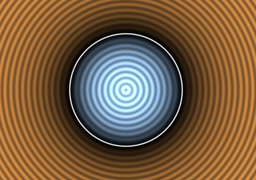
\includegraphics[width=0.5\textwidth]{figures/gfx00.png}
        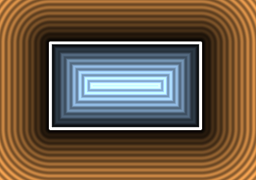
\includegraphics[width=0.5\textwidth]{figures/gfx02.png}
        \caption[SDF of a circle and a box in 2D \cite{iquilezles2}]{SDF of a circle and a box in 2D}
        \label{fig:sdf}
    \end{figure}

    \subsection{Bitonic Sort}

    Bitonic merge sort is a sorting algorithm with a performance complexity of $O(\log^2(n))$. The algorithm can be implemented on the GPU to achieve a massive performance increase by parallelization. In this work, a modified version of the implementation by \href{https://twitter.com/tgfrerer}{@tgfrerer} was used, as shown in the article on his website \cite{bitonic}. The algorithm uses a pattern of comparisons to sort a list of elements in parallel. An example of such a pattern can be seen in illustration \ref{bitonic_sort_pattern}. The algorithm has been modified to use Vulkan's Push Constants to select the type of comparison inside of the shader provided by \href{https://twitter.com/tgfrerer}{@tgfrerer} \cite{bitonic}. Another change is the use of Specialization Constants to set the local workgroup size of the compute shader invocation.

    \begin{figure}[H]
        \begin{center}
            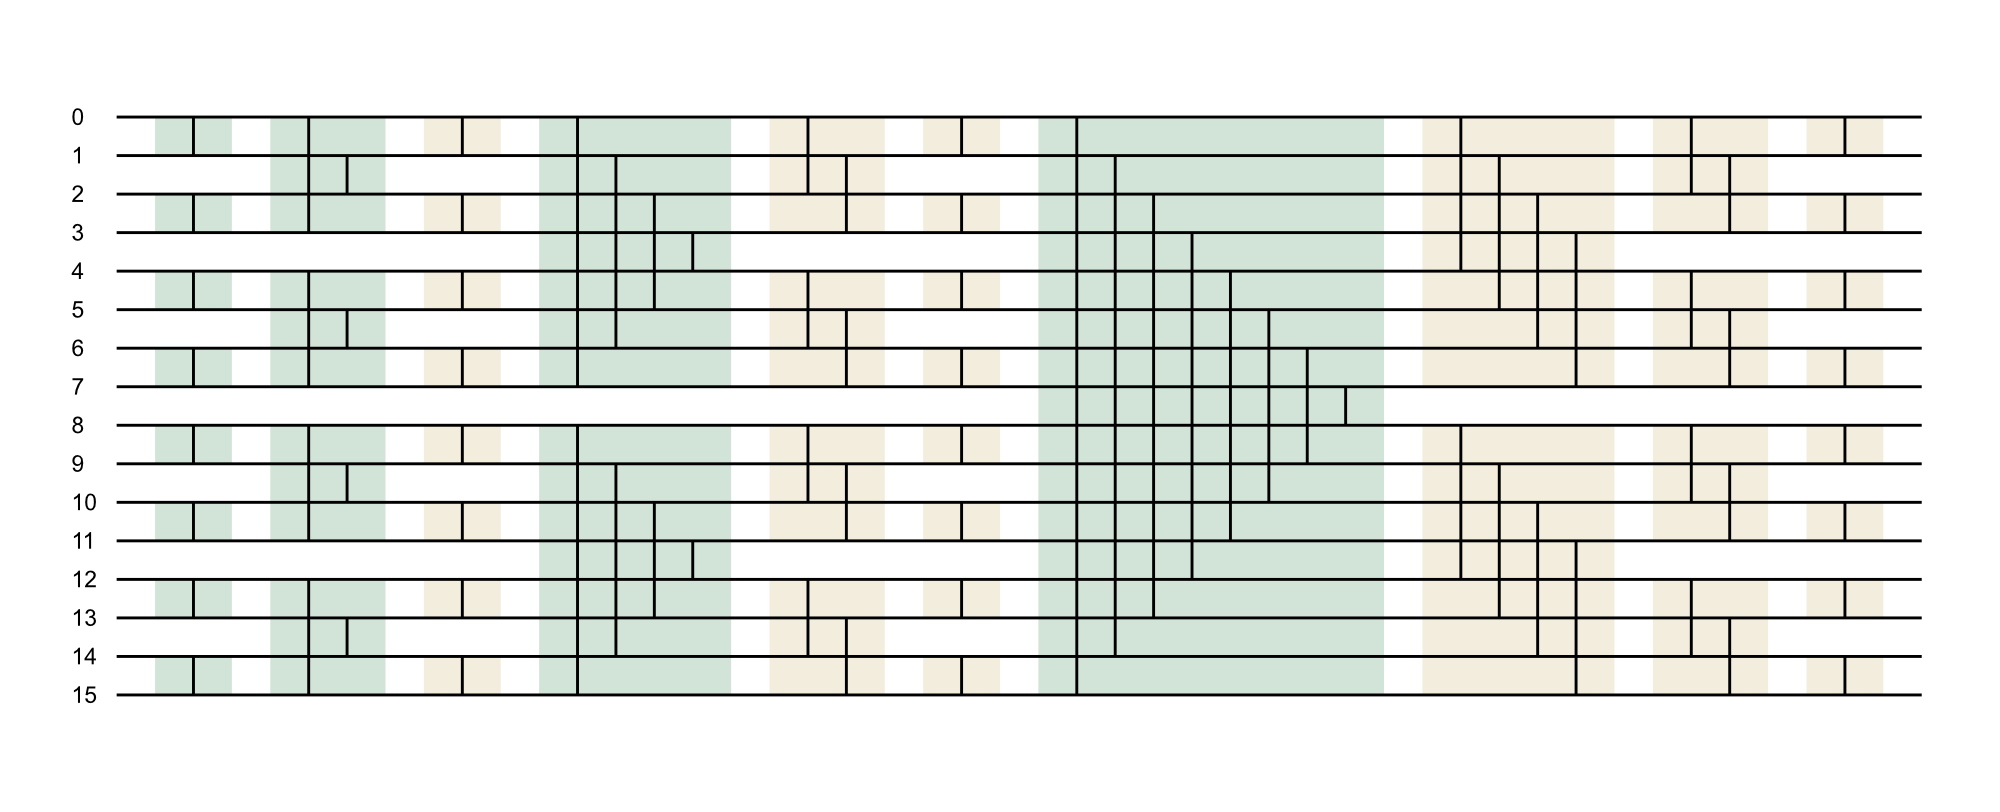
\includegraphics[width=1\textwidth]{figures/bitonic_sort.png}
        \end{center}
        \caption[Sorting diagram for 16 sortable elements. Horizontal lines represent array indices into our array of sortable elements, each vertical line represents one worker thread performing a compare-and-swap operation. \cite{bitonic}]{Sorting diagram for 16 sortable elements. Horizontal lines represent array indices into our array of sortable elements, each vertical line represents one worker thread performing a compare-and-swap operation.}
        \label[fig]{bitonic_sort_pattern}
    \end{figure}

    \pagebreak
    \section{Method} \label{sec:method}
    To understand the implemented algorithms it is neccessary to be familiar with Smoothed Particle Hydrodynamics, which will be explained in this chapter. The purpose and reasoning behind the use of certain libraries and APIs will also be explained.

    \subsection{Smoothed Particle Hydrodynamics}
    Smoothed Particle Hydrodynamics (SPH) is a computational technique widely employed in fluid dynamics and other fields for simulating complex physical phenomena. SPH represents the fluid or material as a collection of discrete particles. Each particle has physical properties such as density, pressure and velocity. 

    These interact through a kernel function $W$ with radius $h$, which smoothes these properties over neighboring particles, allowing for a continuous representation of the material and facilitating the simulation of intricate behaviors, including fluid flow, collision and deformation. An arbitrary field $H$ can be approximated as following, with $m$ being the mass, $x$ and $x_j$ being the position and its neighbor and $\rho$ the density of a particle. \cite{wcsph} 

    \begin{equation}
        H(x) = \sum_j m_j \frac{H_j}{\rho_j} W(|x - x_j|, h)
    \end{equation}

    This concept is then applied to calculate the properties of a given particle. SPH's versatility extends beyond fluids, making it applicable to problems involving granular materials (e.g. \cite{10.2312:LocalChapterEvents:CEIG:CEIG09:011-018}), astrophysics \cite{Springel_2010}, and even solid mechanics \cite{solid_mechanics}. 

    A typical implementation for a kernel function is the cubic spline kernel by Monaghan \cite{doi:10.1146/annurev.aa.30.090192.002551} as shown in figure \ref{fig:kernels}. In this work, a spiky kernel, shown in figure \ref{fig:kernels}, as implemented by Sebastian Lague \cite{seblague} is used, as it provided better results for granular matter. \\

    \begin{figure}[H]
        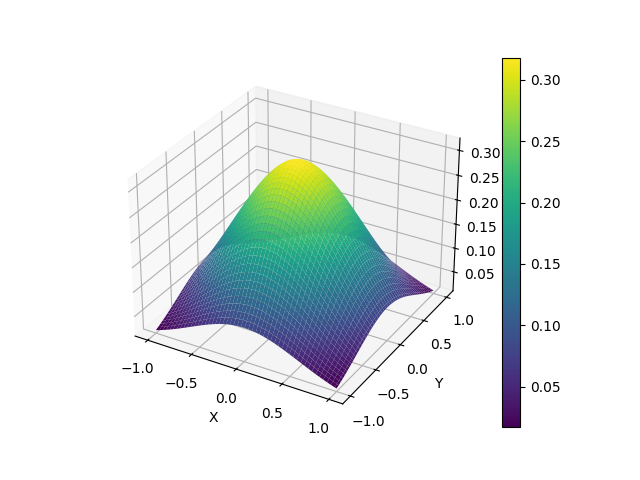
\includegraphics[width=0.5\textwidth]{figures/cubic_spline.png}
        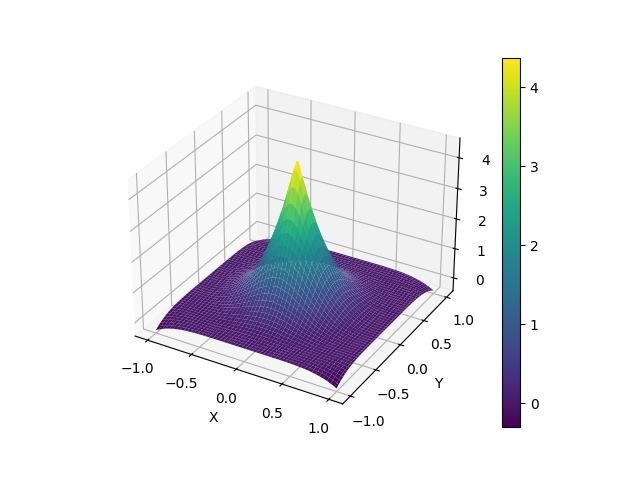
\includegraphics[width=0.5\textwidth]{figures/spiky.png}
        \caption[Kernel functions]{3D representation of a cubic spline kernel function (left) and the in this work utilized spiky kernel function (right)}
        \label{fig:kernels}
    \end{figure}

    There are various methods of smoothed particle hydrodynamics (SPH) each tailored to address different challenges in fluid simulation.

    \subsubsection*{Weakly Compressible SPH}
    Weakly Compressible Smoothed Particle Hydrodynamics (WCSPH) is a variant of the traditional SPH method, where the incompressibility of the Navier-Stokes equation is not as highly enforced, allowing for a more computationally efficient simulation while still capturing the essential fluid behaviors. This approach is particularly useful in scenarios where the fully incompressible SPH formulation might be computationally expensive. It finds a compromise between precision and computational efficiency. This is especially useful in the context of large-scale simulations or real-time applications.\cite{wcsph}

    \subsubsection*{Predictive-Corrective Incompressble SPH} 
    Predictive-Corrective Incompressible SPH (PCISPH) is an advancement in the SPH method, designed to address issues related to incompressibility in fluid simulations. It employs a two-step process where a predictive step estimates particle velocities and a corrective step, which iteratively adjusts these velocities to enforce incompressibility. This technique is particularly useful in scenarios where traditional SPH methods such as WCSPH struggle with maintaining fluid volume conservation, providing more accurate and stable simulations, especially for scenarios involving complex fluid interactions, like fluid splashes or turbulent flows. \cite{10.1145/1576246.1531346}

    \subsubsection*{Implicity Incompressble SPH} \label{sec:iisph}
    Implicit Incompressible Smoothed Particle Hydrodynamics (IISPH) is a variant of the SPH method that also addresses the challenge of maintaining incompressibility in fluid simulations. Unlike traditional SPH methods, IISPH employs an implicit formulation for the pressure term, this will be described in section \ref{sec:pressure}, allowing for larger time steps and improved stability.\cite{6570475} 

    \pagebreak
    \subsection{Libraries \& Technologies}

    \subsubsection*{C++ \& Vulkan}
    When choosing a framework for a fluid simulation using SPH most implementations (for example: \cite{splishsplash} \cite{dualsphysics}) use C++ in combination with OpenMP\cite{openmp} to achieve parallelization, other implementations involve CUDA \cite{cuda} to access the massive parallel compute performance of GPUs \cite{dualsphysics}. For rendering these simulations, dedicated renderers are used. In this implementation Vulkan \cite{vulkan} in combination with C++ 20 is used to simulate and visualize the granular material on the GPU using a combination of compute shaders and the rasterization pipeline. This allows for massive parallel computation of the simulation togehter with the visualization in real time, giving maximum flexibility and extensibility by for example a raytraced visualisation. Vulkan uses SPIRV Shaders, which allows the use of any shading language that can be compiled to it. This work opted for GLSL for its well known C like structure. To make the shader code more readable C style macros were employed.

    \subsubsection*{CMake}    
    CMake \cite{cmake} is a cross-platform build system and project configuration tool and a popular choice in software development, streamlining the build process, enhancing code portability, and offering flexibility in managing diverse project structures and dependencies.

    \subsubsection*{Vulkan Memory Allocator}   
    In contrast to other Graphics APIs Vulkan requires the programmer to do the memory management on the GPU. Vulkan Memory Allocator (VMA)\cite{vma} is employed to achieve efficient management and optimization of GPU memory, simplifying memory allocation and deallocation processes and improving overall performance. 

    \subsubsection*{shaderc}   
    Shaderc\cite{shaderc} is utilized for the compilation and linking of shaders due to its user-friendly interface and simplicity in handling these processes. This enables the user to easily compile the used GLSL shaders to SPIRV for Vulkan to use.

    \subsubsection*{TinyGLTF \& STB Image}  
    In computer graphics, TinyGLTF \cite{tinygltf} is often used for seamless asset loading of 3D models in the Graphic Language Transmission Format (glTF) and STB Image, which is already integrated into TinyGLTF, is favored for its straightforward approach to handling and processing images, both known for their efficiency and ease of use across different applications.

    \subsubsection*{Dear ImGui}
    Dear ImGui\cite{imgui} is a popular immediate mode graphical user interface (GUI) library. It simplifies the process of creating and integrating user interfaces into applications by providing an intuitive and efficient framework and has implementations for nearly every common graphics API and windowing library. It also supports features like multiple viewports and docking elements to them.

    \subsubsection*{GLFW}
    GLFW \cite{glfw} is a widely-used windowing library that simplifies the creation and management of windows, handling user input and facilitating cross-platform development for OpenGL- and Vulkan-based applications.

    \subsubsection*{glm}
    GLM \cite{glm} is a versatile C++ mathematics library designed for graphics programming, providing a comprehensive set of functions and classes for vector and matrix operations commonly used in computer graphics.

    \subsubsection*{TriangleMeshDistance}
    TriangleMeshDistance \cite{trianglemeshdistance} offers a user-friendly programming interface for effortlessly creating signed distance fields of adjustible resolution from 3D meshes. 

    \pagebreak
    \section{Implementation}\label{sec:impl}
    The whole implementation consists of a simple abstraction over the Vulkan API. This speeds up the creation of all required objects, such as buffers, descriptor sets and pipelines. First all the particles were created on the CPU side and stored as a storage buffer on the GPU. This buffer can later be bound as vertex buffer to be used in the rendering. The rigid bodies, the simulation can interact with, were loaded from the glTF files and processed into buffers and textures to be used by a dedicated renderpass. To incorporate them into the simulation, they were converted into a signed distance representation stored as 3D textures. With this, all the major data for the simulation is accesible on the GPU.
    The actual algorithm \ref*{alg:main}, which will be explained on the following pages, consists of 14 different compute shaders, which execute the different steps. First, the particles are grouped into their grid cells and the external force for each particle is set to the gravity. Then the resulting grid entries are sorted. Afterwards the start indices of all cells are determined. After that, the density $\rho$, drag force $F^{drag}$, frictional stress $s$, intermediate velocity $v_{adv}$ and intermediate density $\rho_{adv}$ are calulated in separate shaders. Their purpose will be explained in the following subsections. All steps of the simulation are separated by pipeline barriers to ensure a property has been calculated for all particles before accessing them in the next step. After the computation of the intermediate density $\rho_{adv}$ has been issued, the first command buffer is sent to the GPU for processing and its completion is awaited, as the next steps need to be executed for a dynamic amount of iterations. These iterations consist of computing the required variables for the implicit pressure calculation, such as the displacement due to pressure $d_{ij}p_{j}$ and the predicted pressure $p^{l+1}$ and applying the yield criterion to determine the resulting stress. After these steps have been executed the average density error $\rho_{avg} - \rho_0$ determines if another iteration is required. For this, the sum of density errors is transfered from the GPU to the CPU and divided by the amount of particles. All other computations happen exclusivly on the GPU by accessing the particles stored in the storage buffer. After the IISPH \ref{sec:iisph} iterations are done, the resulting forces are computed and integrated over the elapsed time. In the last step the simulation is visually enhanced by advecting a set of high resolution particles based on the flow of the before computed low resolution behavior and external forces. After this step the storage buffer containing the high resolution particles is bound to a renderpass for drawing and the algorithm starts from the beginning. All steps will now be explained in detail. Starting of with the neighborhood search in line 1 of the algorithm \ref{alg:main} layed out here:
    \begin{algorithm}[H]
        \caption{Full Simulation Frame}
        \label{alg:main}
        \begin{algorithmic}[1]
        \State find neighbors 
        \State compute density $\rho$ 
        \State compute surface normal $n$
        \State compute stress $s$ and drag force $F^{drag}$ 
        \State compute intermediate velocity$v_{adv}$
        \State compute intermediate density $\rho_{adv}$
        \State iteration index $l = 0$
        \While {$l < 2$ $||$ $\rho_{avg} - \rho_0 < \lambda $}
            \State compute $d_{ij}p_{j}$
            \State compute $p^{l+1}$
            \State $p(t) = p^{l+1}$
            \State apply yield criterion 
            \State $l = l+1$
        \EndWhile
        \State compute pressure force $F^p$ and frictional force $F^f$ 
        \State integrate 
        \State advect HR particles 
        \end{algorithmic}
    \end{algorithm}

    \subsection{Neighborhood Search}
    Using the SPH approximation involves finding all neighboring particles within the smooting length $h$. In a naive implementation this means iterating over all other particles and checking their distance to each other. With a runtime of $O(n^2)$ this is not an option for a realtime scenario. To improve the neighborhood search a number of algorithms could be employed. 
    In this implementation a grid based approach has been used, where every particle is first segmented into a spatial grid with cell size of the smoothing length $h$. This provides the possibility to find every neighbor of a given particle, by finding its cell and iterating over its members and all adjacent cells. This severely decreases the amount of particles that have to be checked every frame. 
    To get a list of particles for each cell, all grid entries, consisting of a cell key and a particle ID, are first sorted by the cell key. As this sorting has to be done at the beginning of every frame, it must be done as fast as possible. To achieve this, a parallel sorting algorithm, such as radix sort or in this case bitonic merge sort is used. After the list of grid entries has been sorted, the start of every cells entries has to be found by checking if the cell key of an entry and its predecessor are the same. The starting index of the cell is then stored in an array of length $n$, being the particle count, at the position of the cellkey. This implies that all cell keys have to be within the range $0$ to $(n - 1)$. 
    When iterating over a given cells entries, the entries particle ID is used to check if the particle is within the smoothing length. A cell is found by calculating a particles cell key and the keys of its neighboring cells, and looking up the starting index of that cells entries. The entries can then be iterated until the cell key changes. In the below examples (see Tables \ref{tab:unsorted}, \ref{tab:sorted} and \ref{tab:indices}) a list of 8 grid entries is shown, first in their unsorted state, then after they have been sorted and lastly the list of starting indices of each cell, where $-1$ denotes entries where no cell starts. In the actual implementation unsigned integers are used to represent the starting indices and the maximum unsigned integer is used for empty cells. The implementation of the neighborhood search was inspired by these sources: \cite{psuc} \cite{seblague} \cite{bitonic}
    
    \begin{table}[ht]
        \centering
        \caption{Example of unsorted list of grid entries }
        \begin{tabular}{ l c c c c c c c c }
            Cell key    & 2 & 7 & 5 & 3 & 7 & 7 & 5 & 2 \\ 
            Particle ID & 0 & 1 & 2 & 3 & 4 & 5 & 6 & 7 \\   
        \end{tabular}
        \label{tab:unsorted}
    \end{table}

    \begin{table}[ht]
        \centering
        \caption{Example of sorted list of grid entries }
        \begin{tabular}{ l c c c c c c c c }
            Cell key    & 2 & 2 & 3 & 5 & 5 & 7 & 7 & 7 \\ 
            Particle ID & 0 & 7 & 3 & 2 & 6 & 1 & 4 & 5 \\   
        \end{tabular}
        \label{tab:sorted}
    \end{table}

    \begin{table}[ht]
        \centering
        \caption{Example of list of starting indices }
        \begin{tabular}{ l c c c c c c c c }
            Starting indices    & -1 & -1 & 0 & 2 & -1 & 3 & -1 & 4 \\ 
        \end{tabular}
        \label{tab:indices}
    \end{table}

    This approach allows the grid to have an undefined size as only the amount of particles matters for the creation of it. 

    \subsection{Density}  
    When implementing a SPH simulation the first thing to do is calculate the density $\rho$ of a particle. It is determined by a sum over the neighboring particles. The volume $V$ of each particle within the smoothing length $h$ is multiplied with the density of it and the weighting kernel $ W_{ij} \equiv W(x_i - x_j, h)$. As the volume can be expressed as $V = \frac{m}{\rho}$ we can simplify the equation to only the sum of weighted masses. \cite{wcsph}

    \begin{equation}
        \rho_i = \sum_j m_j W_{ij}
    \end{equation}

    \subsection{Unilateral incompressibility}  
    The next step of the simulation is to compute a pressure that compensates the difference in density between particles. The density and pressure are based on the underlying principle of unilateral incompressibility, which can be expressed in the form: 
    \begin{equation}
        \rho_i \leq \rho_0 \; \bot \;  p \geq 0
    \end{equation}
    This says that the density of a given particle $i$ can not be greater than the rest density of the material and the pressure can not become negative. \cite{10.1145/2019406.2019410}

    \subsection{External forces}
    A change in density can be achieved by applying external forces to the particles. In this simulation a gravitational force and an approximated drag force are employed.
    \subsubsection{Gravity}
    Gravity is given as a fixed acceleration in a given direction in 3D space. Multiplied with the weight of a given particle we get a force, which we can use in our integration step.
    \subsubsection{Drag}
    As an additional force that approximates the interaction with air, a drag force $F^{drag}$ was applied, which uses a simplified implementation of the drag by Gissler et al.\cite{10.1016/j.cag.2017.09.002}. For this the relative velocity difference of a particle to the surrounding air is computed and its length squared. 

    \begin{equation}
        \label{eq:v_rel}
        v^2_{i,rel} = |v_a - v_i|^2\ \frac{v_a - v_i}{|v_a - v_i|}
    \end{equation}

    The velocity of the air $v_a$ can be set to 0, to represent still air, or could be taken from a velocity field of some kind. Computing the drag force to apply to each particle, involves determining the crosssectional area $A_i$ of a particle. This is approximated by the area of a circle. Then the actual area exposed to oncoming air needs to be determined. For this a cone which is defined by the direction of the relative velocity difference and a set angle is used to check if there are any other particles that shield the current particle from the air. This is done by a dot product of the relative velocity difference and the vector to the neighboring particles, which returns the angle between them. To not only get a boolean value for the shielding, an occlusion value is introduced, which is set to the smallest angle between neighboring particles in the cone. This value is then subtracted from 1 and added to the drag formulation as weight $\Omega$. Further parameters for equation \ref{eq:f_drag} by Gissler et al. \cite{10.1016/j.cag.2017.09.002} are $\rho_a$ the density of the air or the medium that surrounds the particles and $C_{D,i}$ the drag coefficient for shape of the particle. The whole formula is then composed as: 

    \begin{equation}
        F^{drag}_i = \frac{1}{2}\rho_a v^2_{i,rel} C_{D,i}  \Omega  A_i
        \label{eq:f_drag}
    \end{equation}

    The deformation of a particle by the oncoming air is left out in this implementation.

    To have not only the air influence the granular material, but have the air also flow over and around it, another compute pass was added to calculate the surface normal $n$ for each particle, using the gradient of the so called smoothed color field $\nabla c^s$ as proposed by Müller et al. \cite{10.5555/846276.846298}:

    \begin{equation}
        n = -\nabla c^s
    \end{equation}

    with $\nabla c^s$ being computed as: 

    \begin{equation}
        \nabla c^s = \sum_j m_j \frac{1}{\rho_j} \nabla W_{ij}
    \end{equation}

    With this approximation for the surface of the granular matter, an approximate air flow along the surface was calculated by projecting the incoming air velocity onto the plane, defined by the surface normal:

    \begin{equation}
        v_{a, i} = v_{a} - v_{a} \cdot n_i
    \end{equation}

    The rough approximation for the air flowing over the surface of the granular matierial $v_{air, i}$, was then plugged into equation \ref{eq:v_rel}. \\
    This yields an effect where a sandpile blown by wind towers on the windward side (direction the wind is coming from) and flattens on the leeward side (the wind averted side). On the ridge between them, the particles detach from the pile and are fly through the air. The effect is shown in figure \ref{fig:blow} and is comparable to the behavior seen at dunes.

    \begin{figure}[H]
        \centering
        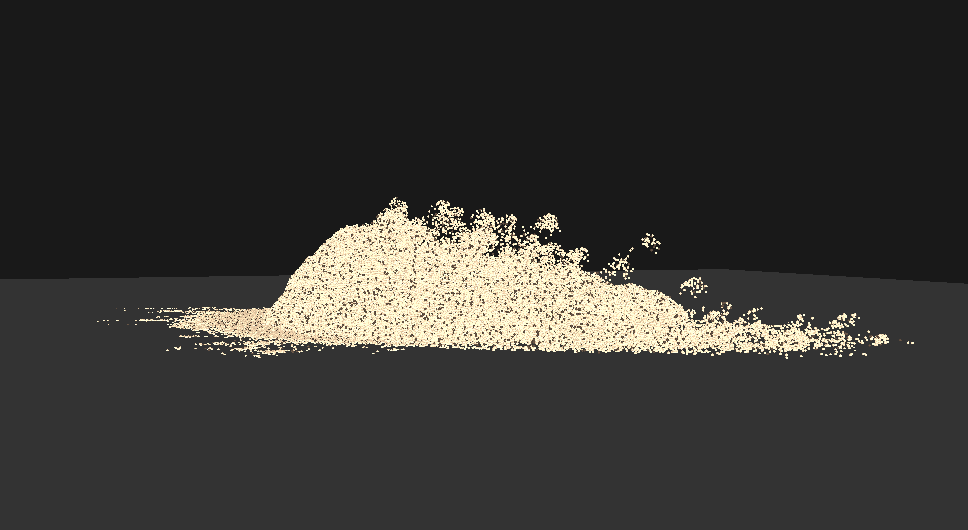
\includegraphics[width=0.7\textwidth]{figures/wind_blown_pile.png}
        \caption[A pile of sand blown by wind coming from the left]{A pile of sand blown by wind coming from the left}
        \label{fig:blow}
    \end{figure}


    \subsection{Strain \& Stress}
    
    To simulate friction between the particles of the granular material, the strain $\varepsilon$ needs to be calculated first. It measures the deformation of a material under external forces and is represented as a tensor of rank 3. This involves determining the velocity gradient $\nabla u_i$ by an outer product of the velocity $u_j$ with the kernel gradient $\nabla W_{ij}$. 
    
    \begin{equation}
        \nabla u_i = \sum_j V_j \nabla W_{ij} u_j^T
    \end{equation}

    The strain is then computed as:
    \begin{equation}
        \varepsilon = \frac{1}{2} (\nabla u_i + \nabla u_i^T)
    \end{equation}

    Particles can withstand a certain amount of strain before slipping occures. This is expressed by the stress tensor. For the computation of the frictional stress a parameter $D$, which relates the frictional stress $s$ to the dissipation of strain is calculated as:

    \begin{equation}
        D_i = \frac{2 m_i^2 \Delta t}{\rho_i^2} \sum_j \frac{1}{\rho_j} \nabla W_{ij}  \nabla W_{ij}^T
    \end{equation}
    
    The parameter can be precomputed for a prototype particle with a filled neighborhood, to make the computation more efficient.
    The stress is obtained by multiplying the strain tensor with the inverse of $D$. 
    
    \begin{equation}
        s_i = D^{-1} \varepsilon
    \end{equation}

    For most dry granular materials there is no or neglegible cohesion (The tendency of particles to stick to each other). This means that the mean hydrostatic stress $s_{i, hydrostatic}$ can be subtracted from the stress computed above, enforcing a traceless deviatoric stress $s_{i, deviatoric}$, which is further referred to as $s_i$. 

    \begin{equation}
        s_{i, hydrostatic} = \frac{1}{2} \Tr s_i 
    \end{equation}
    \begin{equation}
        s_{i, deviatoric} = s_i - s_{i, hydrostatic} 
    \end{equation}

    Cohesion can be handled similarly to friction, as demonstrated by Aludan et al. in their work SPH Granular Flow with Friction and Cohesion \cite{10.1145/2019406.2019410}.

    The amount of friction applied is limited by the pressure. This is expressed by the Drucker-Prager yield criterion:

    \begin{equation}
        ||s_i|| \leq p_i \alpha
    \end{equation}

    \begin{equation}
        \alpha = \sqrt{2} \sin \Theta
    \end{equation}

    Where $\alpha$ is the frictional coefficient for an angle of repose $\theta$ (the maximum angle a material can pile before slipping) and $||s_i||$ the frobenius norm of $s_i$. The yield constraint can be approximated in a piecewise linear manner by applying it to each component of $s$. \cite{10.1145/2019406.2019410} \cite{10.2312:PE:vriphys:vriphys12:053-060} \cite{10.2312:LocalChapterEvents:CEIG:CEIG09:011-018} \cite{10.1145/1866158.1866195}

    \subsection{Pressure} \label{sec:pressure}
    In traditional SPH methods the pressure $p$ is calculated by an equation of state like the ideal gas equation \cite{wcsph}
    \begin{equation}
        p_i = k * (\rho_i - \rho_0)
    \end{equation}
    or Tait's equation \cite{wcsph}
    \begin{equation}
        p_i = B ((\frac{\rho_i}{\rho_0})^{\gamma} - 1)
    \end{equation}
    where $k$, $B$ and $\gamma$ are parameters controlling the stiffness of the pressure calculation, which means the scaling from the density error to the resulting pressure.
    PCISPH then tries to minimize the mean density error by doing multiple iterations, correcting the applied pressure. As WCSPH does not provide good enough incompressibility for stable friction calculations and PCISPH can take a lot of iterations to converge, IISPH \ref{sec:iisph} was chosen for this implementation, as it provides pressures that result in a very small mean density error after only a few iterations and supports larger timesteps than other variants of SPH.

    The IISPH \ref{sec:iisph} implemetation consist of two parts. The first being the advection of the velocities and densities and the second, the iterations to solve for the pressure. For the advection all external forces are summed up and the particle velocities are advanced in time to get an intermediate velocity $v_i^{adv}$. \cite{6570475}

    \begin{equation}
        F_i^{adv} = F^g + F_i^{drag}
    \end{equation}

    \begin{equation}
        v_i^{adv} = v_i + \Delta t \frac{F_i^{adv}}{m_i}
    \end{equation}

    The intermediate velocity is then used to calculate predicted density $\rho_i^{adv}$ for all particles. \cite{6570475}

    \begin{equation}
        \rho_i^{adv} = \rho_i + \Delta t \sum_j m_j v_{ij}^{adv} \nabla W_{ij}
    \end{equation}
    
    At this point the base pressure to use for the upcoming steps is set to $p_{last} = 0.5p$ \cite{6570475}. The following equation is then used to determine the pressure values.

    \begin{equation}
        p_i^{l+1} = (1 - \omega) p_i^l + \omega \frac{1}{a_{ii} * \Delta t^2} (\rho_0 - \rho_i^{adv} - \Delta t^2 \psi)
    \end{equation}

    Here $l$ is the index of the current iteration of the algorithm. The factor $\omega$ is called the relaxation factor and is set ot $0.5$ as this value yields the best results \cite{6570475}. $a_{ii}$ is a coefficient that is computed per particle as: 

    \begin{equation}
        a_{ii} = \sum_j m_j (d_{ii} - d_{ji}) \nabla W_{ij}
    \end{equation}

    , with $d_{ii}$ and $d_{ji}$ being the same parameter for particle $i$ and $j$ respectivly, which is computed as:

    \begin{equation}
        d_{ii} = \Delta t^2 \sum_j -\frac{m_j}{\rho_i^2} \nabla W_{ij}
    \end{equation}

    The before used value $\psi$ is calculated as shown below:

    \begin{equation}
        \psi = \sum_j m_j (\sum_j d_{ij}p_j^l - d_{jj}p_j^l - \sum_{k \neq i} d_{jk}p_k^l) \nabla W_{ij}
    \end{equation}

    \begin{equation}
        \sum_{k \neq i} d_{jk}p_k^l = \sum_{k} d_{jk}p_k^l - d_{ji}p_i^l 
    \end{equation}

    , where $\sum_j d_{ij}p_j^l$ is computed every iteration as:

    \begin{equation}
        \sum_j d_{ij}p_j^l = \Delta t^2 \sum_{k} -\frac{m_j}{\rho_j^2} p_j^l \nabla W_{ij}
    \end{equation}

    Now, the yield can be testet with the new pressure and the new density is predicted as:

    \begin{equation}
        \rho_i^{l+1} = |p * a_{ii} * \Delta t^2 - (\rho_0 - \rho_i^{adv} - \Delta t^2 \psi)| + \rho_0
    \end{equation}

    It is then used to determine the overall average density error of all particles. For this the Vulkan Shader Atomic Float Extension is utilized to sum up the density error over all particles on the GPU and then divide it by the number of particles on the CPU. This value then determines if another iteration is required to achieve the desired threshold. Always at least two iterations are performed before using the average density error as a termination criterion. The implementation of the whole pressure calculation was guided by the open source library SPlisHSPlasH \cite{splishsplash}. For more details on how the IISPH \ref{sec:iisph} algorithm works, see the paper, Implicit Incompressible SPH, by Ihmsen et al. \cite{6570475}.

    \subsection{Internal Forces}
    
    For the calculation of the pressure force of a given particle the SPH concept is applied again \cite{10.2312:PE:vriphys:vriphys12:053-060}. 

    \begin{equation}
        F_i^p = -m_i \sum_{j \neq i} m_j (\frac{p_i}{\rho_i^2} + \frac{p_j}{\rho_j^2})  \nabla W_{ij}
    \end{equation}
    
    A similar formulation can be used to determine the frictional force of that particle \cite{10.2312:PE:vriphys:vriphys12:053-060}.

    \begin{equation}
        F_i^f = -m_i \sum_{j \neq i} m_j (\frac{s_i}{\rho_i^2} + \frac{s_j}{\rho_j^2})  \nabla W_{ij}
    \end{equation}

    

    \subsection{Integration}
    For the integration of the simulation a simple Euler integration was used. It could be exchanged for a more advanced integrations scheme such as Leap-Frog or Verlet.
    \begin{equation}
        v_i(t + \Delta t) = v_i^{adv} + \Delta t \frac{F_i^p}{m_i}
    \end{equation}
    \begin{equation}
        x_i(t + \Delta t) = x_i + \Delta t v_i(t + \Delta t)
    \end{equation}

    \subsection{Boundary Handling}
    
    \subsubsection*{Particle-Based Approaches}
    Most implementations of SPH use the concept of Akinci et al. \cite{boundary_handling} when implementing boundary handling and rigid body interactions. The first implementation of this work also used this method, but later the concept of volume maps was adopted due to multiple advantages. The idea behind the method of Akinci et al. \cite{boundary_handling} is to represent boundaries and rigid bodies by sampling their surface or volume with one or more layers of particles as shown in figure \ref{fig:particle_boundary}, which can then be incoporated into the normal particle simulation. For static objects the boundary particles are not integrated in time. For dynamic rigid bodies, the particles representing them collect the counteracting forces, they excert onto the fluid. The collected forces can then be summed up and integrated by a rigid body physics solver.
    This method presents some drawbacks. One of them being the amount of particles required to sample large or complexe 3D models in the scene, which then have to be checked for each neighboring fluid particle. \cite{10.1145/3359566.3360077} \cite{10.2312:PE:vriphys:vriphys12:053-060} \cite{boundary_handling} \cite{10.1145/2185520.2185558}

    \begin{figure}[H]
        \centering
        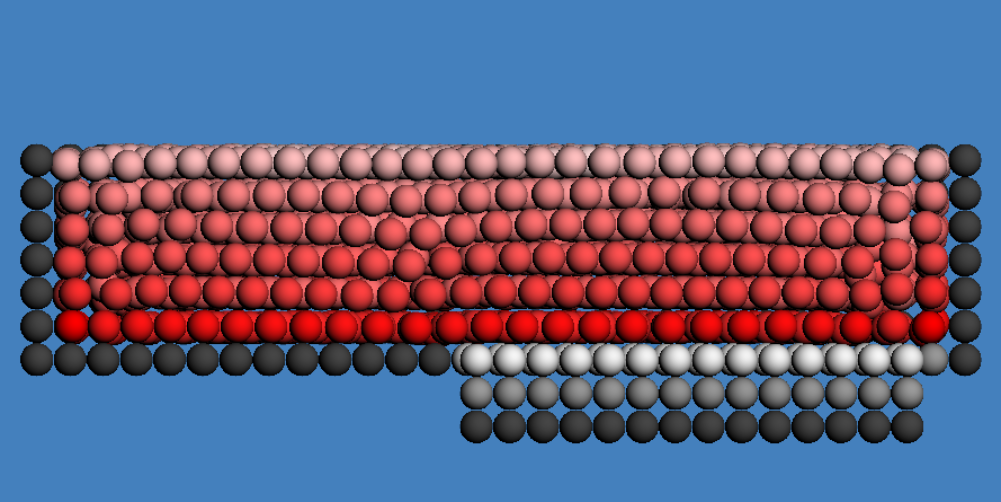
\includegraphics[width=0.5\textwidth]{figures/particle_boundary.png}
        \caption[Example of a 2D boundary sampled with particle. On the left one layer and on the right a version with multiple layers. \cite{10.1145/2185520.2185558}]{Example of a 2D boundary sampled with particle. On the left one layer and on the right a version with multiple layers.}
        \label[fig]{fig:particle_boundary}
    \end{figure}

    \subsubsection*{Volume Maps}
    In this implementation the concept of Volume Maps is employed. They are an implicit boundary representation, inspired by the density maps concept. They use signed distance functions to determine the volume of the intersection of the kernel function around a particle and the boundary. For this, the boundary or bounding box of any arbitrary mesh is extended by the kernel radius and then sampled on a grid with a set resolution. Here the TriangleMeshDistance library \cite{trianglemeshdistance} is used to create a signed distance representation of any triangle based mesh. For each sample a vector to the nearest point on the surface of the object is stored aswell as the intersection volume $V_B$, which is calculated by the signed distance $\Phi$, treated by a cubic extension function $\gamma^*$, to get a continuos differentiable function, which results in a smooth transition at $x = h$. \cite{10.1145/3359566.3360077}

    \begin{equation}
        V_b(x) = \int_{N(x)}\gamma^*(\Phi(x'))dx'
    \end{equation}

    \begin{equation}
        \gamma^*(x) = 
        \begin{cases}
            \frac{C(x)}{C(0)},& \text{if } 0 < x < h \\
            1,& \text{if } x \leq 0 \\
            0,              & \text{otherwise}
        \end{cases}
    \end{equation}

    For this cubic extension function the cubic spline kernel $C(x)$ \cite{doi:10.1146/annurev.aa.30.090192.002551} is used. The use of this function does not enforce the use of the same function for the SPH approximation, where any kind of kernel function can be used. \cite{10.1145/3359566.3360077}
    The grid is then stored as a 32-bit 4-channel floating point 3-dimensional image and uploaded to the GPU. As Vulkan does not support arrays of 3D images, as it does for 2D textures, the Descriptor Indexing Extension has to be used, to allow for multiple 3D textures being bound dynamically. When sampling the texture in the shader, the nearest position on the surface and the intersection volume can be determined using only one texture read access instead of iterating all neighboring boundary particles as done in the particle-based approach. After transforming the volume map from its texture space into world space inside of the shader, a smooth value for both required properties is determined by the sampler. These values can the be used in any of the above mentioned equations, by substituting the mass for the determined volume $V_b$ and the reference density $\rho_0$ of the simulated material, resulting in the following equations for the density:

    \begin{equation}
        \rho_i = \sum_b V_b \rho_0 W_{ib}
    \end{equation}

    for the pressure force:

    \begin{equation}
        F_i^p = -m_i \sum_{b} V_b \rho_0 (\frac{p_i}{\rho_i^2}) \nabla W_{ib}
    \end{equation}

    and for the frictional force:

    \begin{equation}
        F_i^f = -m_i \sum_{b} V_b \rho_0 (\frac{s_i}{\rho_i^2}) \nabla W_{ib}
    \end{equation}


    For the calculation of the resulting boundary forces only the pressure and stress of the particle is used, other than in the calculation of the forces between particles, where both particles contribute to the force. At this point the boundary forces can be applied to the actual rigid body, the volume map represents, to allow for two way coupling of the simulation and the boundaries. In the following illustration a slice of a volume map can be seen.

    \begin{figure}[H]
            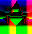
\includegraphics[width=0.5\textwidth]{figures/volume_map_slice_xyz.png}
            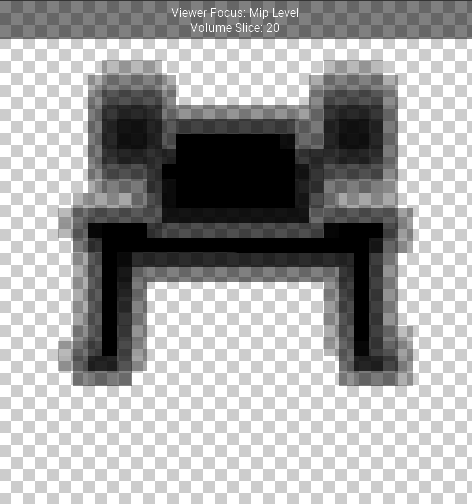
\includegraphics[width=0.5\textwidth]{figures/volume_map_slice_w.png}
        \caption[Slice of a volume map for a dump truck model, showing the nearest point and volume. Extracted using Nvidia Nsight Graphics.]{Slice of a volume map for a dump truck model, showing the nearest point and volume. Extracted using Nvidia Nsight Graphics.}
        \label[fig]{volume_map}
    \end{figure}


    \subsection{Upsampling}
    \label{sec:upsampling}
    As granular matter consists of vast numbers of grains, simulating them all as individual particles, would not only make the computational cost and memory consuption extremly high, but would also result in a very restricted time step due to the Courant-Friedrichs-Lewy (CFL) condition, which determines the maximum viable timestep for a numerical stable simulation. To achieve real time results, the simulation is done for a set of low-resolution (LR) particles which approximate the granular flow, which are then upsampled to another set of high-resolution (HR) particles. \cite{10.2312:PE:vriphys:vriphys12:053-060}
    A volume around each low-resolution particle is initially sampled with a special pattern of high-resolution particles, which tries to minimize the effect of clumping. For this, each LR particles bounding box is sampled with $N$ HR particles. Then 6 bounding box sized volumes, offset in both positive and negativ X, Y and Z direction by the particle radius, are also sampled with $N$ particles, resulting in $7N$ HR particles for each LR particle. Figure \ref{fig:sampling} shows a 2D example of this method.

    \begin{figure}[H]
        \centering
        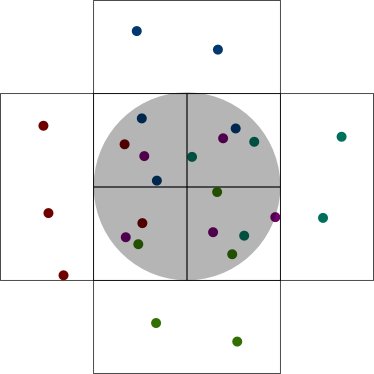
\includegraphics[width=0.5\textwidth]{figures/sampling.png}
        \caption[2D Example of the HR sampling of a LR particle (grey area) with $N = 5$. Particles of the same region are colored the same to show the denser sampling of the reagion in the area of the LR particle.]{2D Example of the HR sampling of a LR particle (grey area) with $N = 5$. Particles of the same region are colored the same to show the denser sampling of the reagion in the area of the LR particle.}
        \label[fig]{fig:sampling}
    \end{figure}


    After the above described algorithm is executed on the low-resoltion particles, the high resolution particles are advected based on the velocity field of the low-resolution simulation. This is again done by the SPH concept, but with a different smoothing length $h_{HR}$ which is set to $h_{HR} = 3h_{LR}$. To find the velocity of a HR particle a distance based weight $w$ is introduced.

    \begin{equation}
        w(\delta_{ij}) = \max(0, (1 - \frac{\delta_{ij}^2}{h_{HR}^2})^3)
    \end{equation}

    In this equation $i$ refers to a high-resolution particle and $j$ to a low-resoltion particle or a boundary and $\delta_{ij}$ to the distance between them. The velocity is the computed as the weighted average velocity over the neighboring LR particles.\cite{10.2312:PE:vriphys:vriphys12:053-060}

    \begin{equation}
        v_i^*(t + \Delta t) = \frac{1}{\sum_j w(\delta_{ij})}\sum_j w(\delta_{ij})v_j
    \end{equation}

    As the LR particles should be able to not only follow the flow of the granular material, but react to gravity when there are no LR particles in its range, a blending weight $\eta$ is introduced, to define the contributions of the simulation and external forces. The final velocity of each HR particle is then computed as:

    \begin{equation}
        v_i(t + \Delta t)  = (1 - \eta)v_i^*(t + \Delta t) + \eta(v(t) + \Delta t \frac{F^g}{m})
    \end{equation}

    where $\eta$ is:

    \begin{equation}
        \eta = 
        \begin{cases}
            1 - \arg \max_j w(\delta_{ij}),& \text{if } \frac{\arg \max_j w(\delta_{ij})}{\sum_j w(\delta_{ij})} \geq 0.6 \\
            1 - \arg \max_j w(\delta_{ij}),& \text{if } \arg \max_j w(\delta_{ij}) \leq w(r_{LR}) \\
            0,              & \text{otherwise}
        \end{cases}
    \end{equation}

    The constant $0.6$ is an empirically tested value for the above defined high-resolution smoothing length \cite{10.2312:PE:vriphys:vriphys12:053-060}. 
    
    To prevent the HR particles from penetrating the boundaries multiple different approaches have been investigated. For these, an additional loop over all volume maps is performed. The first approach tried to modify the $\eta$ value, by multiplying it with 1 minus the dot product of the external force and the vector to the boundary, clamped between 0 and 1, which prevented the particles from falling through, but made a lot of particles stick to vertical boundaries. For the next approach each boundaries weight was computed by applying the weighting kernel $w(d_{ib})$ with $d_{ib}$ being the distance to the boundary. Then a weighted velocity $w(d_{ib}) v_i(t + \Delta t)$ was computed and subtracted from $v_i(t + \Delta t)$. This also prevented the particles from falling through boundaries and had a lot less sticking occuring.

    Additionaly the position of the particle is offset to counteract any penetration, by first determining the signed distance to the boundary, using a dot product of the distance to the boundary $x_{i,b}$ and the surface normal $n$ and adjusting this distance by the low-resolution particle radius and then offseting the position by this distance $\Delta x_{i,b}$ if it is negative. The computation of the final particle position $x_{final}$ is summarized as:
    \begin{equation}
        \Delta x_{i,b} = (x_i - x_b) \cdot n
    \end{equation}
    \begin{equation}
        x_{final} = 
        \begin{cases}
            x + (\Delta x_{i,b} + r_{LR}) n,     & \text{if } x_{i,b} < 0 \\
            x,              & \text{otherwise}
        \end{cases}
    \end{equation}
    
    \subsection{Visualization}
    As the visualisation was not the main focus of this work, it is kept simple. To visualize the simulation, all particles were rendered as instanced meshes, as the number of particles to draw can become quite large and in this way all of them can be rendered in just one draw call. A detailed explanation of instanced rendering can be found on in source \cite{instancing}. The rigid bodies were rendered by drawing each node of the model with its associated material, as its own draw call and were shaded with a simple diffuse lighting model.

    \subsection{User interaction}
    For the user to experience the simulation in 3D space, a camera controller has been implemented, that allows to explore the simulation from every angle. The simulation can be paused and reset to its initial state by buttons provided via the user interface. It also allows to modify some of the simulations parameters, such as the density, gravity or air velocity. Another purpose the UI serves is to provide infomation about the perfomance, such as timing, iteration count or framerate. The UI has been implemented in a way that allows the user to rearange all the windows, inside and outside of the main window. There for the docking and multi-viewport features of Dear ImGui have been utilized. The UI can be seen in figure \ref{fig:ui}

    \begin{figure}[H]
        \centering
        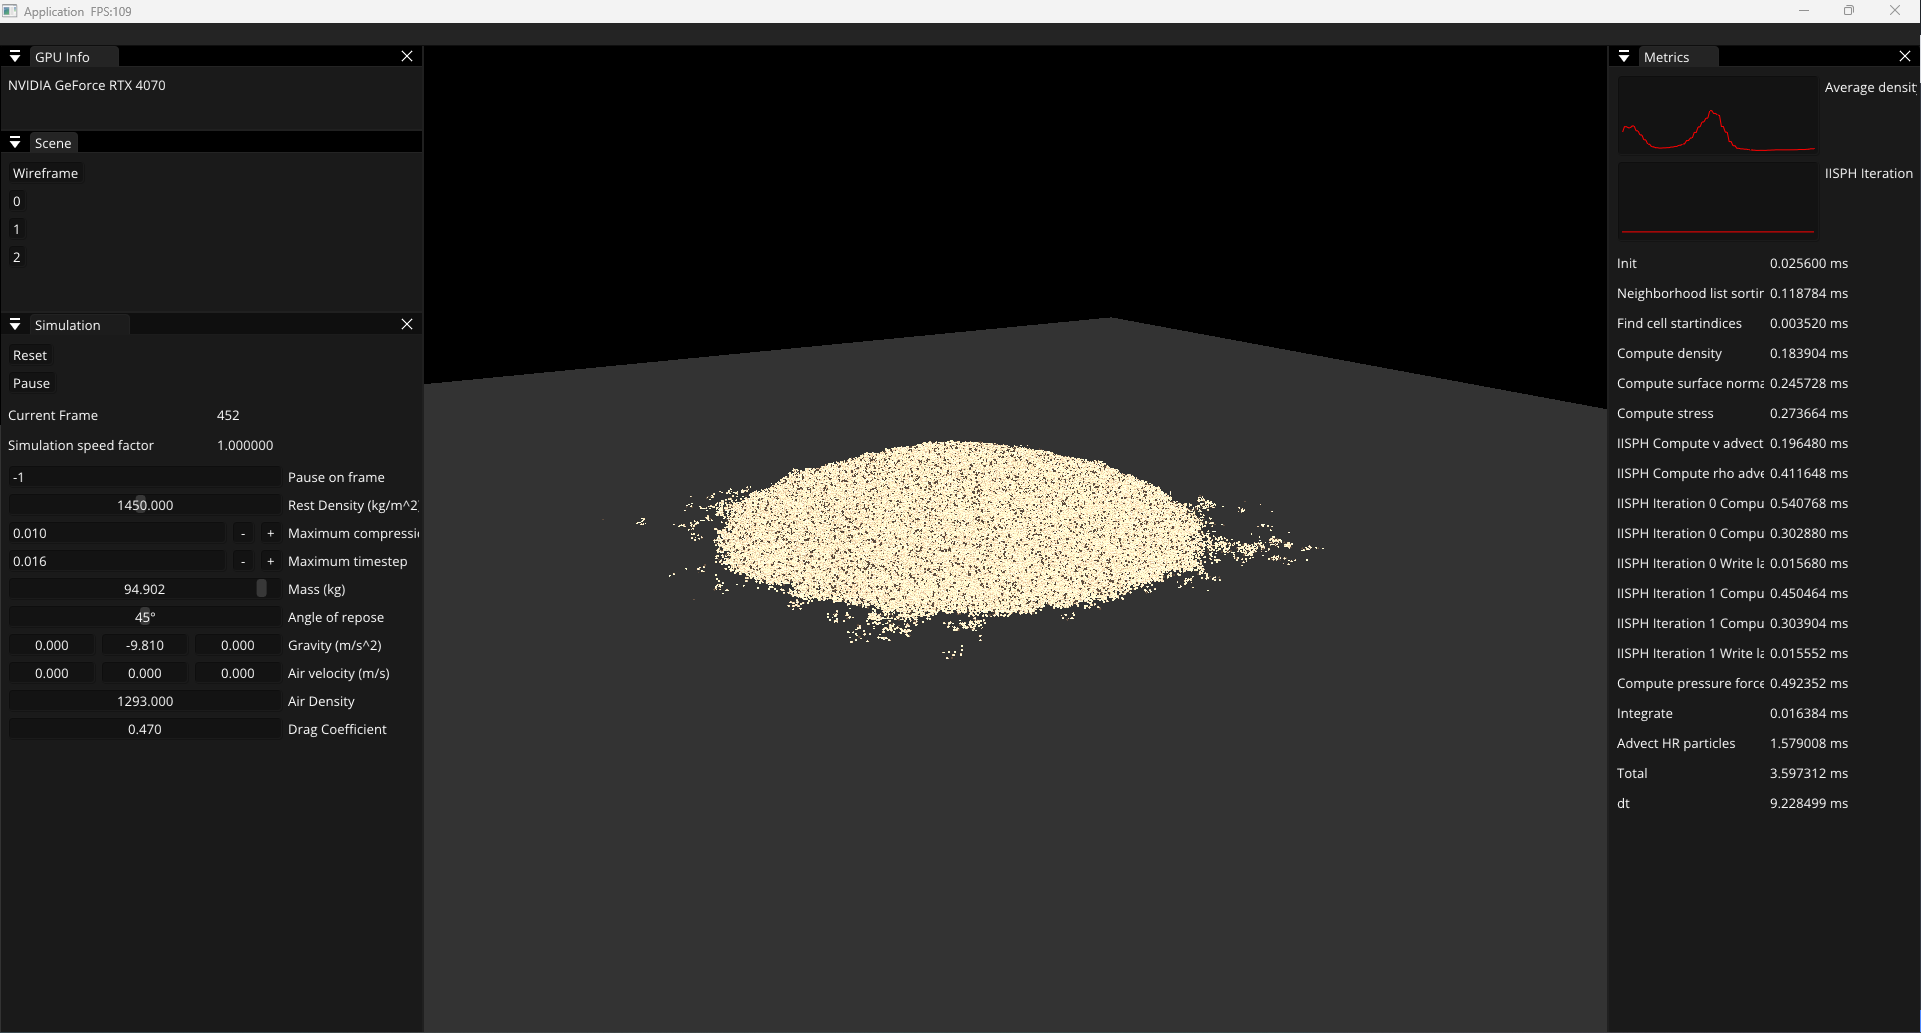
\includegraphics[width=1\textwidth]{figures/ui.png}
        \caption[Screenshot of the User interface.]{Screenshot of the User interface.}
        \label[fig]{fig:ui}
    \end{figure}

    \pagebreak
    \section{Conclusion \& Future Work}  \label{sec:end}
    % intro
    When comparing this work with some of the related works presented in section \ref{sec:related}, the major difference lies in the time a frame takes to compute, as the other works mostly run on CPU only. This implementation combines the basic concepts, of simulating granular matter using SPH, from the works of Ihmsen et al. \cite{10.2312:PE:vriphys:vriphys12:053-060} and Alduan et al. \cite{10.1145/2019406.2019410} with the boundary handling introduced by Bender et al. \cite{10.1145/3359566.3360077}, the IISPH \ref{sec:iisph} algorithm by Ihmsen et al. \cite{6570475} for the pressure calculation and the approximation of drag forces by Gissler et al. \cite{10.1016/j.cag.2017.09.002}. All of this results in a simulation, that achieves the same effects as in the mentioned papers, while running with interactable framerates. \\
    % piles
    The simulation achieves the accumulation of stable piles with different angles of repose (the angle where the material starts to slip), while keeping them stable for an extended amount of time, as shown in figure \ref{fig:piles}.
    \begin{figure}[H]
        \centering
        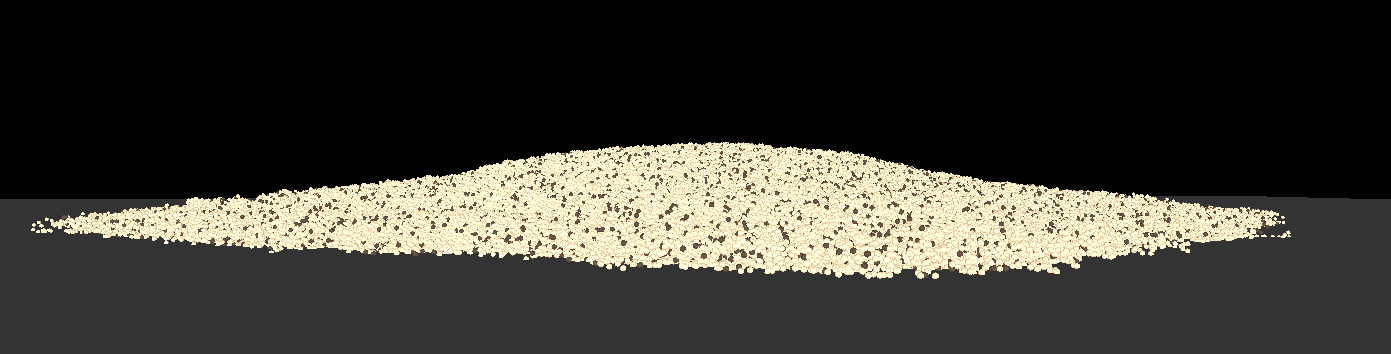
\includegraphics[width=0.60\textwidth]{figures/pile_30_1000.png}
        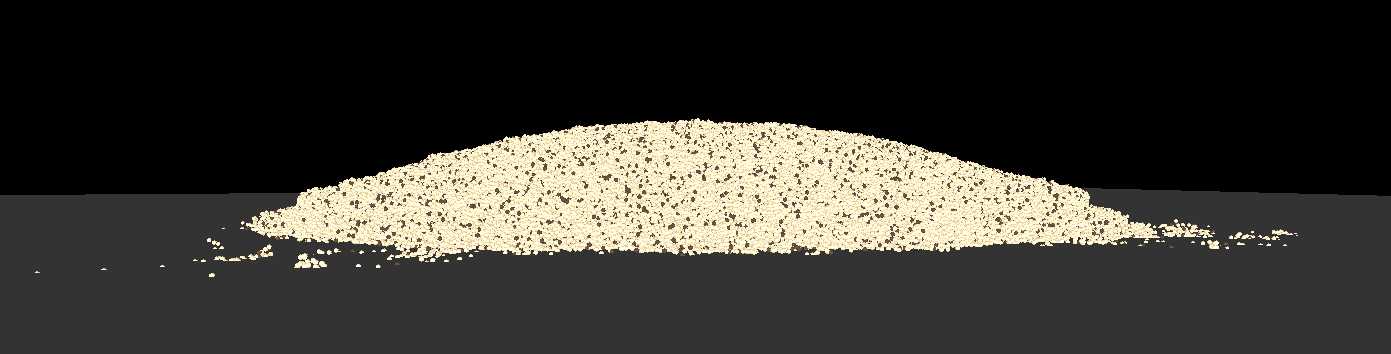
\includegraphics[width=0.60\textwidth]{figures/pile_45_1000.png}
        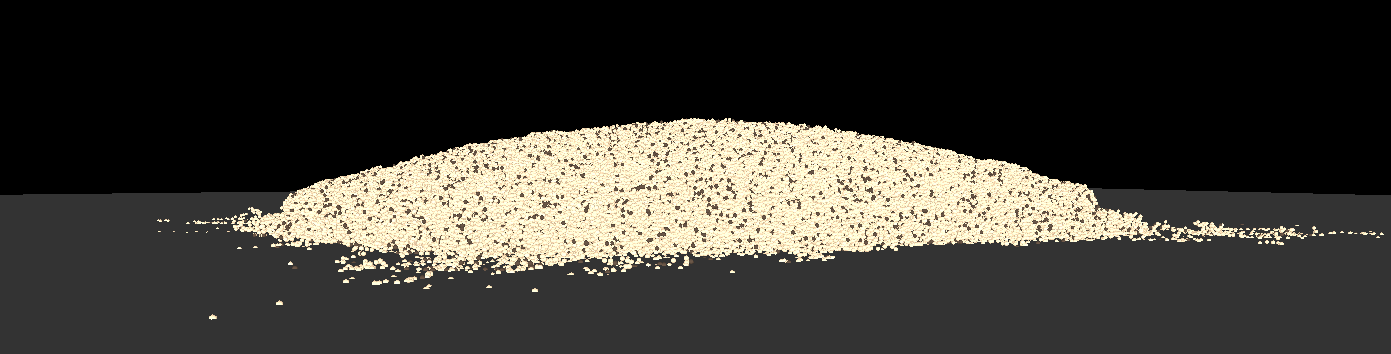
\includegraphics[width=0.60\textwidth]{figures/pile_60_1000.png}
        \caption[Three piles with different angles of repose, simulated for 1000 frames.]{Three piles with different angles of repose (fromt top to bottom: 30°, 45°, 60°), after 1000 frames. The difference between the second and third image is not that noticable anymore, due to the \enquote{melting} of the piles.}
        \label[fig]{fig:piles}
    \end{figure}
    After a longer simulation time the piles will eventually melt down, due to a \enquote{bubbling} effect. Its cause or a solution to it was not found in this implementation. The problem can be improved by lowering the default maximum allowed compression of 1\%, which was found to be a good compromise between performance and accuracy. This maximum compression is choosen 10 times larger than in the work of Ihmsen et al \cite{6570475}, which might be part of the problem. The maximum timestep was set to 16ms as this results in a framerate of minimum 60 frames per second, while keeping the required iterations in an order of magnitude that can be computed within that timeframe. This value is 4 times higher than in the before mentioned paper \cite{6570475}. These values were determined for a simulation with 8192 low resolution and about 500000 high resolution particles for the piling scenario. For other scenarios the optimal settings may vary.\\
    % IISPH
    These large simulation timesteps are only possible because of the IISPH (\ref{sec:iisph}) algorithm, as the CFL (\ref{sec:upsampling}) condition, which determines the maximum viable timestep based on the simulation parameters, would only allow few or even sub millisecond timesteps with WCSPH or PCISPH. Another improvement might be the implementation of a divergence free solver, as proposed by Bender and Koschier in their paper Divergence-Free Smoothed Particle Hydrodynamics, as it achieved even better perfromance in their tests than IISPH \ref{sec:iisph} \cite{10.1145/2786784.2786796}.
    % volume maps
    The above mentioned \enquote{bubbling} effect is amplified when combining the large compression of 1\% and the large timestep of 16ms with low resolution volume maps, as they can not handle complex objects well. Creating higher resolution volume maps improves this by some margin, but introduces longer loading times and higher memory consumption. 
    The longer loading times could be countered by parallelization or precomputing the volume maps and loading them from files.
    To improve the memory consumption, the representation of the rigid body model could be separated into multiple volume maps with resolutions according to the complexity of the part or to exclude large empty areas on concave objects. Combined with some kind of hierarchical respresentation of the object, the sample time for one rigid body should not increase significantly.
    Another problem the volume maps might have introduced is a visual "step" between the first and the second layer of particles above the floor, as the volume maps representation of the floor is completely flat, in contrast to a floor that was sampled with boundary particles. This is especially noticable on the low resolution representation as shown in figure \ref{fig:layer_step}. This problem was not solvable by applying the modifications to the volume maps approach by Bender et al. in their work, Implicit Frictional Boundary Handling for SPH \cite{9123549} but may be by another approach by Band et al.\cite{10.1145/3180486}. Due to time constraints, this approach remains to be studied in a future implementation.
    \begin{figure}[H]
        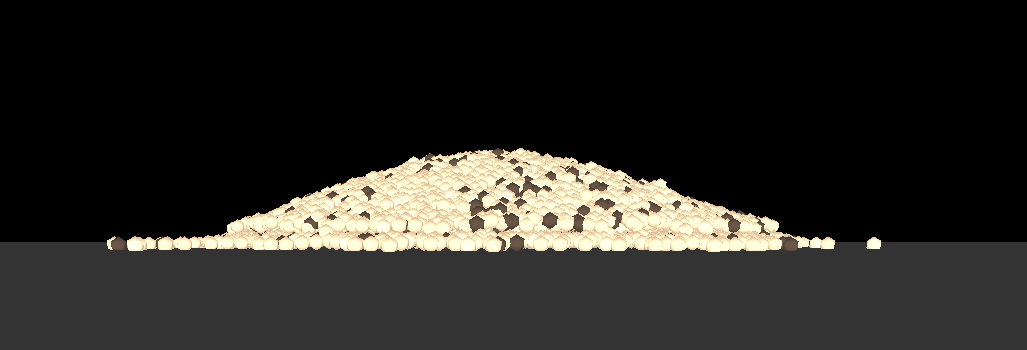
\includegraphics[width=0.5\textwidth]{figures/layer_step.png}
        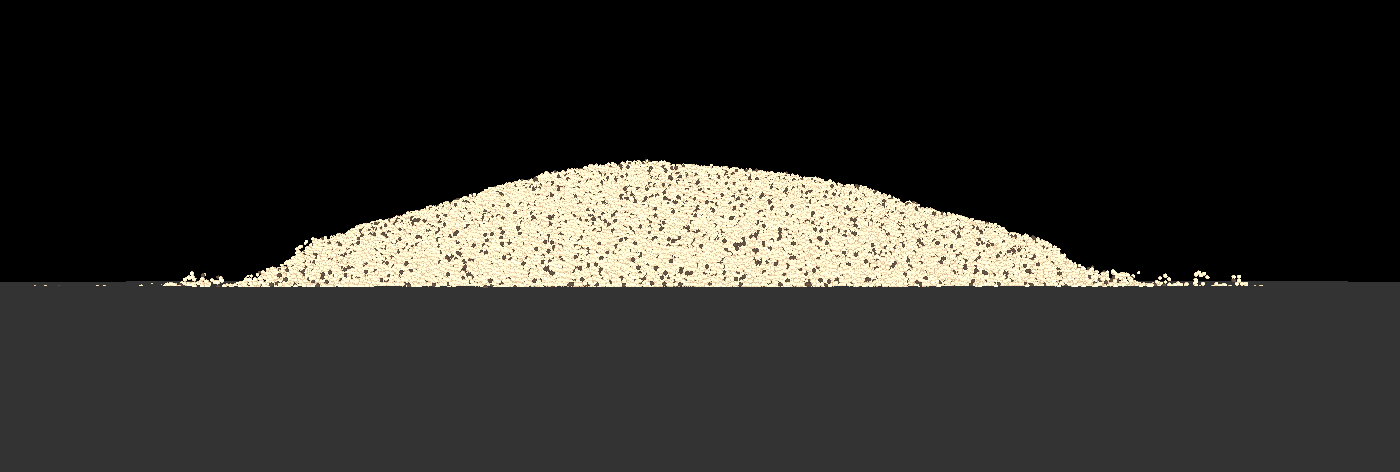
\includegraphics[width=0.5\textwidth]{figures/layer_step_hr.png}
        \caption[Example of the step between the first and the second layer of particles above ground. On the left with LR particles and on the right with HR particles]{Example of the step between the first and the second layer of particles above ground. On the left with LR particles and on the right with HR particles}
        \label[fig]{fig:layer_step}
    \end{figure}
    % upsampling
    % Through the upsampling of the low resolution simulation a visually plausible representation of vast amounts of granular material, comparable to other papers, is achieved. 
    A major problem that Ihmsen et al. \cite{10.2312:PE:vriphys:vriphys12:053-060} already tried to solve by their upsampling approach, is the clumping of high resolution particles, which is still visible. 
    Another problem were particles falling through boundaries, which was countered by the approach presented in section \ref{sec:upsampling}. This introduced another problem, which is the sticking of particles to some shapes as visible in illustration \ref{fig:sticking}. 
    
    \begin{figure}[H]
        \centering
        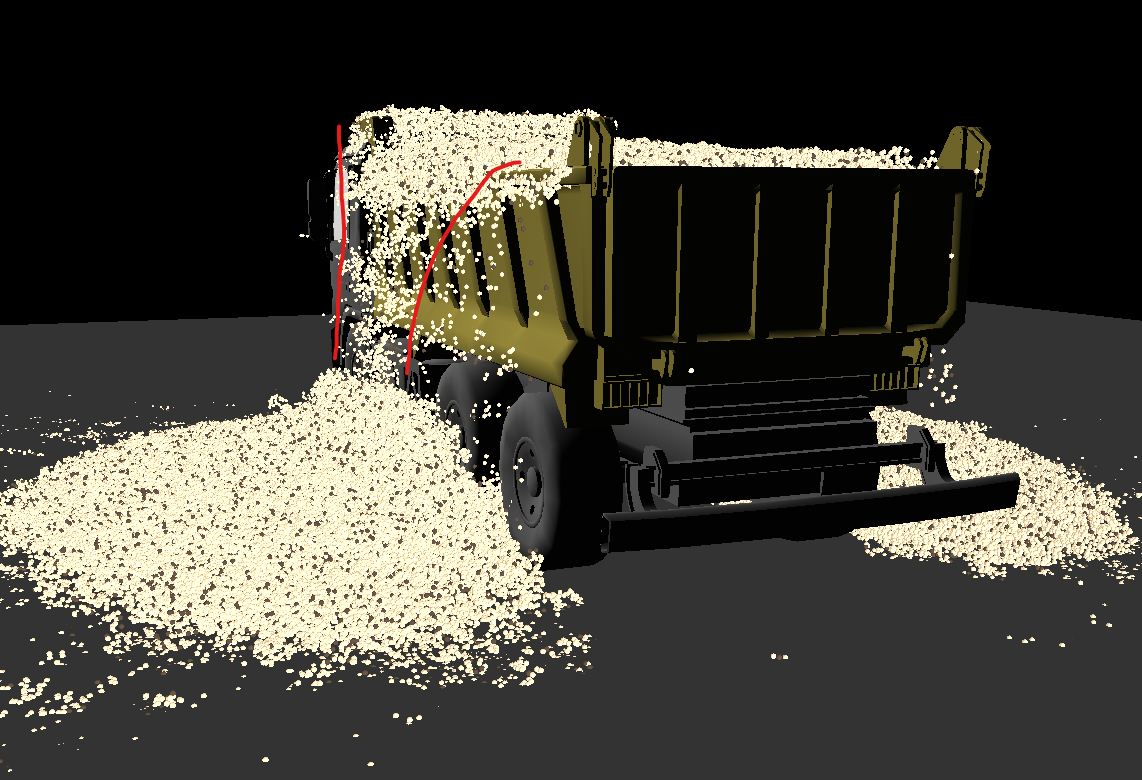
\includegraphics[width=0.7\textwidth]{figures/sticking.png}
        \caption[Example of high resolution particles sticking to the wall of a dump truck.]{Example of high resolution particles sticking to the wall of a dump truck. The particles between the red lines are still overflowing from the dump truck. The particles outside the red lines are sticking to the wall.}
        \label[fig]{fig:sticking}
    \end{figure}
    % two way coupling
    One feature missing from this implementation compared to others is two-way coupling, as the simulation only reacts to static boundaries and does not influence them. This could be implemented in the future by collecting the forces for each rigid body and feeding them into a dedicated solver. \\
    % perfromance
    The performance of the simulation is mostly limited by the upsampling step, as it has to approximate the velocity field for all HR particles, by iterating of all neighboring LR particles. This steps takes 50\% of the computation time for the before mentioned amount of particles. For this process, it would make sense to store the velocity field of the low-resolution particles into a texture to sample it for every high resolution particle instead of looping overall neighbors. This might be an idea for future implementations, as it does no longer follow the SPH principle fully.\\
    The scale of the simulation is smaller than in other implementations. Compared to the implementation of Ihmsen et al. \cite{10.2312:PE:vriphys:vriphys12:053-060}, which has been the main reference for this work, the amount of LR particles for their bulldozer example was 38 000 particles, upsampled to 1.4 mio particles, whereas this implementation consists of 8000 and 0.5 mio respectively. The computation time for their example is at least 2.5 seconds for each frame, while this implementation achieves visually comparable result, just with fewer particles in under 16 miliseconds.\\
    % conclusion
    In conclusion, this work has achieved its goal of exploring the feasibility of a Smoothed Particle Hydrodynamics simulation for granular matter, despite encountering limitations of SPH. However, due to time constraints and limitations of the choosen technique the resulting simulation may not be fully suitable for a physically correct simulation of granular matter in realtime. By combining the used approach with ideas from other methods, such as the Material Point Method \cite{BARDENHAGEN2000529}, Position-Based Dynamics\cite{10.2312:egt.20151045} or other techniques involving multiple grids \cite{Shao:2022:Multigrid} or AI \cite{sanchezgonzalez2020learning}, a physically correct simulation of granular matter in realtime might be possible. 

    The code for this project can be found at:\\
    \url{https://github.com/andre-neder/granular-matter-sph}.
    \pagebreak
    \listoffigures
    \pagebreak
    \printunsrtglossary[type=symbols,style=long]
    \pagebreak
    \printbibliography
\end{document}